% Editable native annotations around unchanged verified IDE photographs.
\par
\begin{figure}[htbp]
  \centering
  \newsavebox{\MARSfirtieregistersBox}
  \sbox{\MARSfirtieregistersBox}{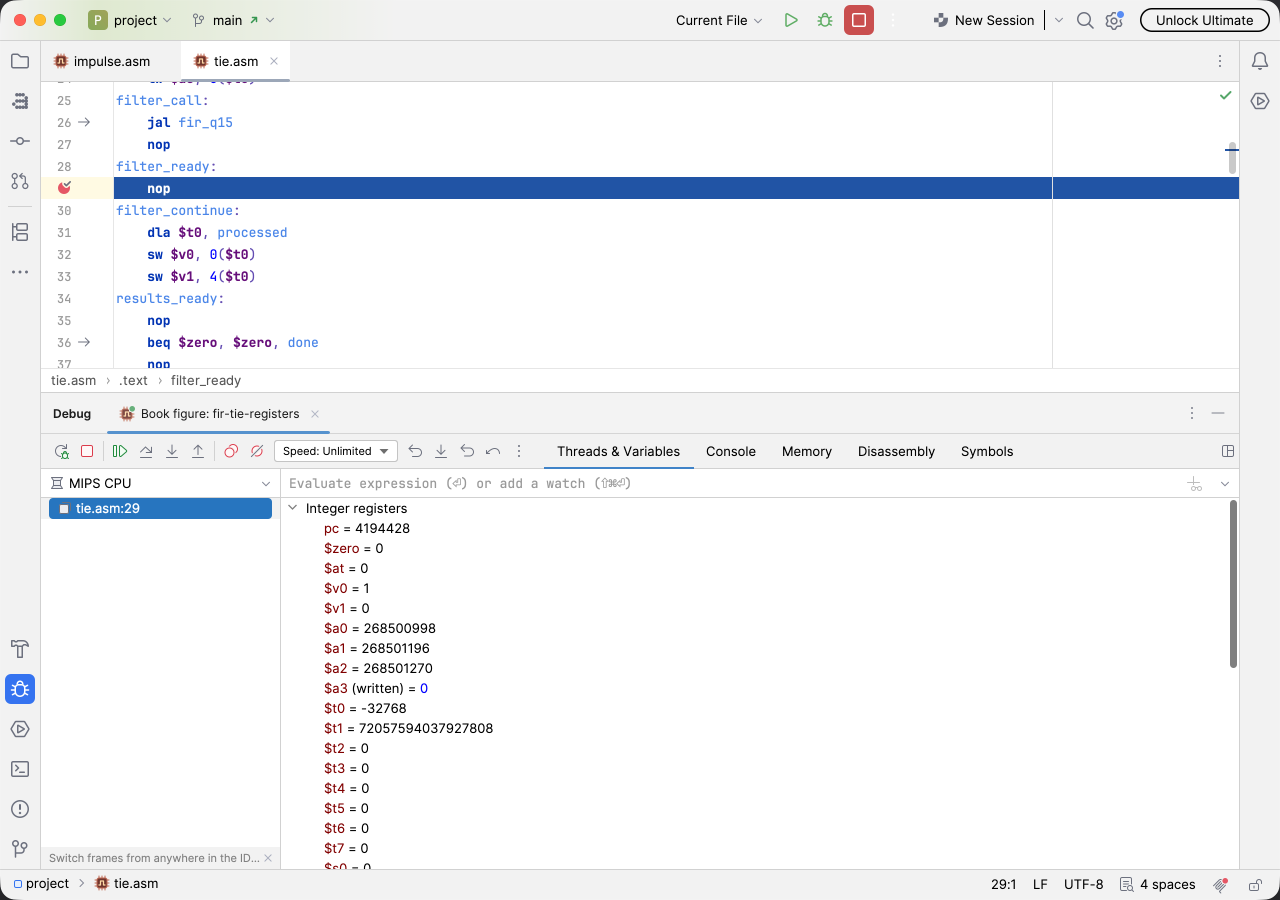
\includegraphics[artifact]{book/captures/021-fixed-point-fir/f03/registers.png}}
  \newsavebox{\MARSfirtieinputBox}
  \sbox{\MARSfirtieinputBox}{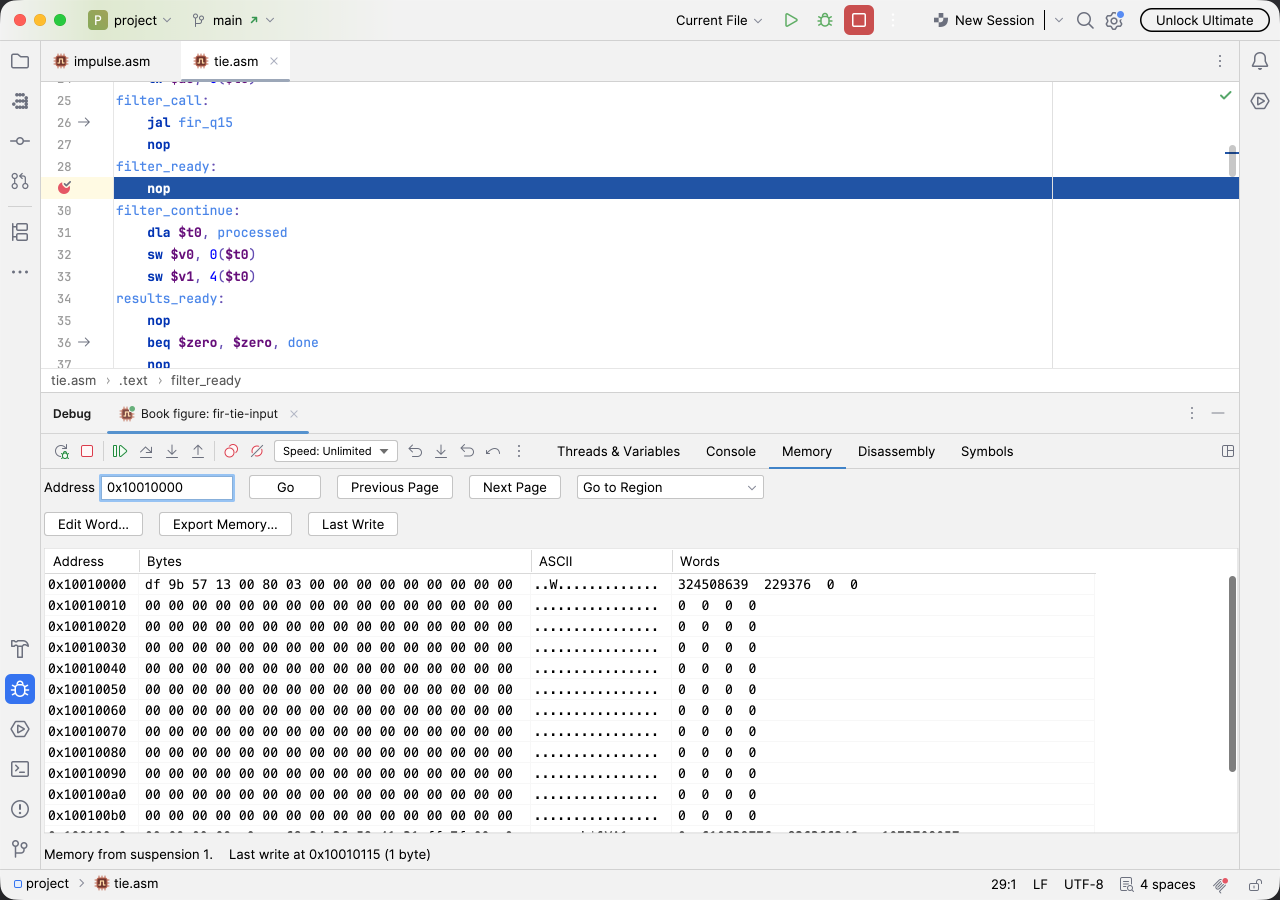
\includegraphics[artifact]{book/captures/021-fixed-point-fir/f03/input.png}}
  \newsavebox{\MARSfirtiecoefficientsBox}
  \sbox{\MARSfirtiecoefficientsBox}{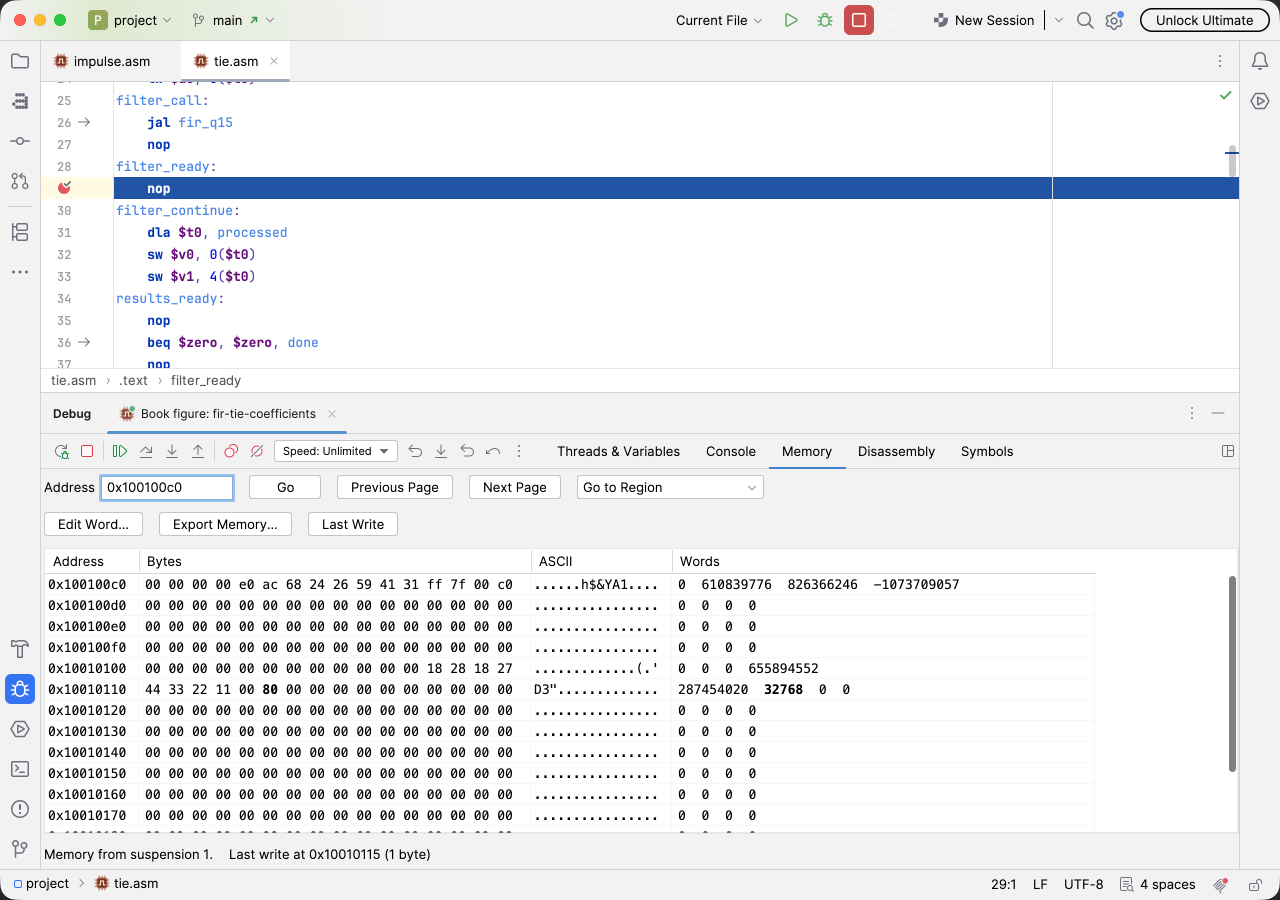
\includegraphics[artifact]{book/captures/021-fixed-point-fir/f03/coefficients.png}}
  \newsavebox{\MARSfirtieoutputBox}
  \sbox{\MARSfirtieoutputBox}{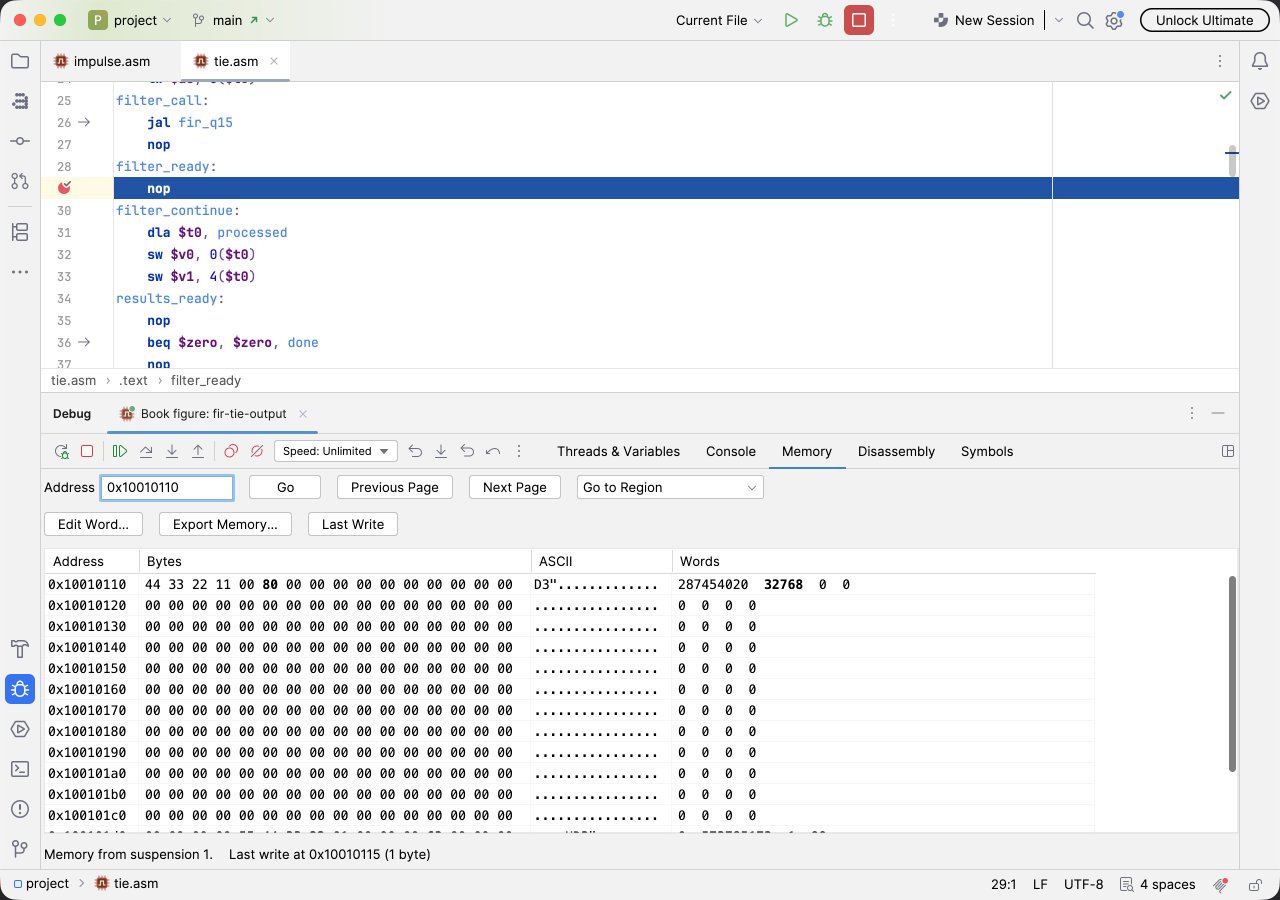
\includegraphics[artifact]{book/captures/021-fixed-point-fir/f03/output.png}}
  \newsavebox{\MARSfirtiecallerBox}
  \sbox{\MARSfirtiecallerBox}{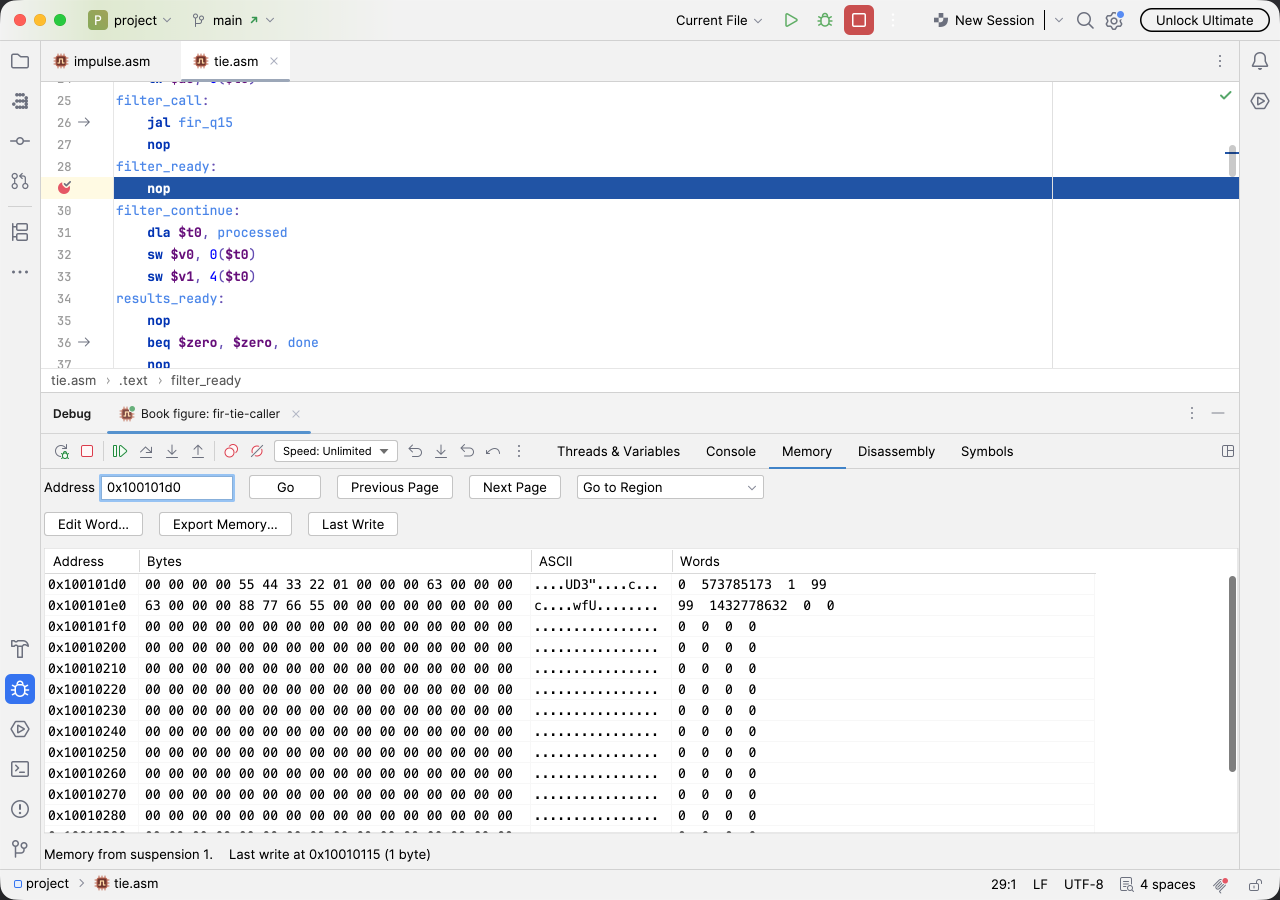
\includegraphics[artifact]{book/captures/021-fixed-point-fir/f03/caller.png}}
  \edef\MARSfirtiesourceLeft{\the\dimexpr0.036718750\wd\MARSfirtieregistersBox\relax}
  \edef\MARSfirtiesourceBottom{\the\dimexpr0.774444444\ht\MARSfirtieregistersBox\relax}
  \edef\MARSfirtiesourceRight{\the\dimexpr0.713281250\wd\MARSfirtieregistersBox\relax}
  \edef\MARSfirtiesourceTop{\the\dimexpr0.170000000\ht\MARSfirtieregistersBox\relax}
  \edef\MARSfirtieregistersLeft{\the\dimexpr0.246093750\wd\MARSfirtieregistersBox\relax}
  \edef\MARSfirtieregistersBottom{\the\dimexpr0.312222222\ht\MARSfirtieregistersBox\relax}
  \edef\MARSfirtieregistersRight{\the\dimexpr0.553906250\wd\MARSfirtieregistersBox\relax}
  \edef\MARSfirtieregistersTop{\the\dimexpr0.640000000\ht\MARSfirtieregistersBox\relax}
  \edef\MARSfirtieinputLeft{\the\dimexpr0.034375000\wd\MARSfirtieinputBox\relax}
  \edef\MARSfirtieinputBottom{\the\dimexpr0.311111111\ht\MARSfirtieinputBox\relax}
  \edef\MARSfirtieinputRight{\the\dimexpr0.584375000\wd\MARSfirtieinputBox\relax}
  \edef\MARSfirtieinputTop{\the\dimexpr0.608888889\ht\MARSfirtieinputBox\relax}
  \edef\MARSfirtiecoefficientsLeft{\the\dimexpr0.034375000\wd\MARSfirtiecoefficientsBox\relax}
  \edef\MARSfirtiecoefficientsBottom{\the\dimexpr0.311111111\ht\MARSfirtiecoefficientsBox\relax}
  \edef\MARSfirtiecoefficientsRight{\the\dimexpr0.584375000\wd\MARSfirtiecoefficientsBox\relax}
  \edef\MARSfirtiecoefficientsTop{\the\dimexpr0.608888889\ht\MARSfirtiecoefficientsBox\relax}
  \edef\MARSfirtieoutputLeft{\the\dimexpr0.034375000\wd\MARSfirtieoutputBox\relax}
  \edef\MARSfirtieoutputBottom{\the\dimexpr0.334444444\ht\MARSfirtieoutputBox\relax}
  \edef\MARSfirtieoutputRight{\the\dimexpr0.584375000\wd\MARSfirtieoutputBox\relax}
  \edef\MARSfirtieoutputTop{\the\dimexpr0.608888889\ht\MARSfirtieoutputBox\relax}
  \edef\MARSfirtiecallerLeft{\the\dimexpr0.034375000\wd\MARSfirtiecallerBox\relax}
  \edef\MARSfirtiecallerBottom{\the\dimexpr0.311111111\ht\MARSfirtiecallerBox\relax}
  \edef\MARSfirtiecallerRight{\the\dimexpr0.584375000\wd\MARSfirtiecallerBox\relax}
  \edef\MARSfirtiecallerTop{\the\dimexpr0.608888889\ht\MARSfirtiecallerBox\relax}
  \begin{tikzpicture}[alt={Six annotated panels at filter_ready show one output and zero clipped. The first inputs are minus 32768 and three; the first coefficients are 32767 and minus 16384, with all remaining codes zero. Their exact scaled sum is minus 32768.5, which rounds toward positive infinity at the tie to minus 32768. Stored output is 00 80 and caller result words remain 99.}]
    \node[anchor=north west,inner sep=0,font=\small\bfseries] (source-title) at (6mm,0) {Next instruction at this boundary};
    \node[anchor=north west,inner sep=0] (source) at ([yshift=-1mm]source-title.south west) {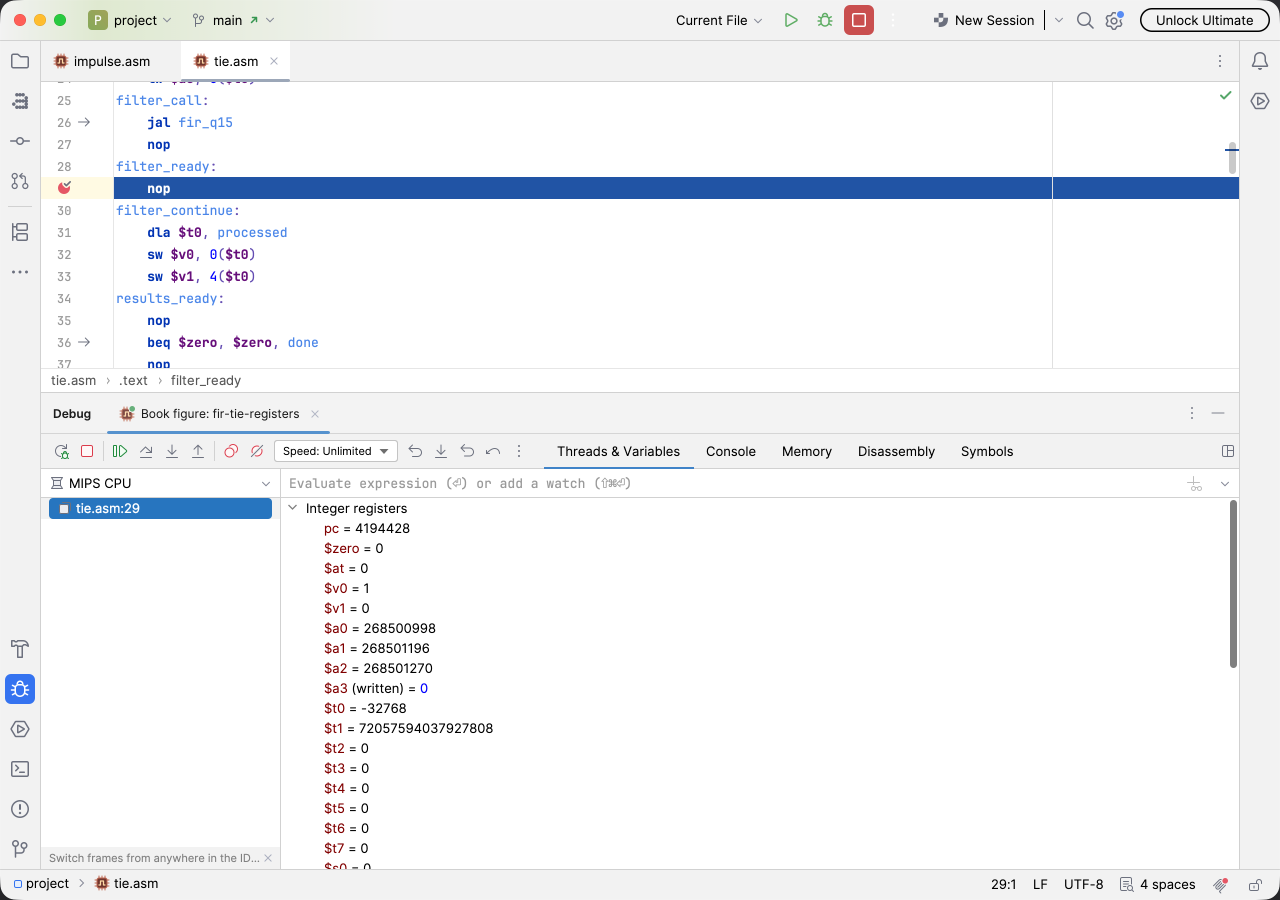
\includegraphics[width=0.54\linewidth,artifact,trim={\MARSfirtiesourceLeft{} \MARSfirtiesourceBottom{} \MARSfirtiesourceRight{} \MARSfirtiesourceTop{}},clip]{book/captures/021-fixed-point-fir/f03/registers.png}};
    \begin{scope}[shift={(source.south west)},x={($(source.south east)-(source.south west)$)},y={($(source.north west)-(source.south west)$)}]
      \draw[black,line width=0.7pt] (0.215625000,0.080000000) rectangle (0.384375000,0.520000000);
      \node[draw=black,fill=white,circle,inner sep=1.5pt,font=\footnotesize] at ($(0.215625000,0.520000000)+(-3mm,0)$) {1};
    \end{scope}
    \node[anchor=north west,inner sep=0,font=\small\bfseries] (registers-title) at (0.58\linewidth,0 |- source-title.north) {Register values at this boundary};
    \node[anchor=north west,inner sep=0] (registers) at ([yshift=-1mm]registers-title.south west) {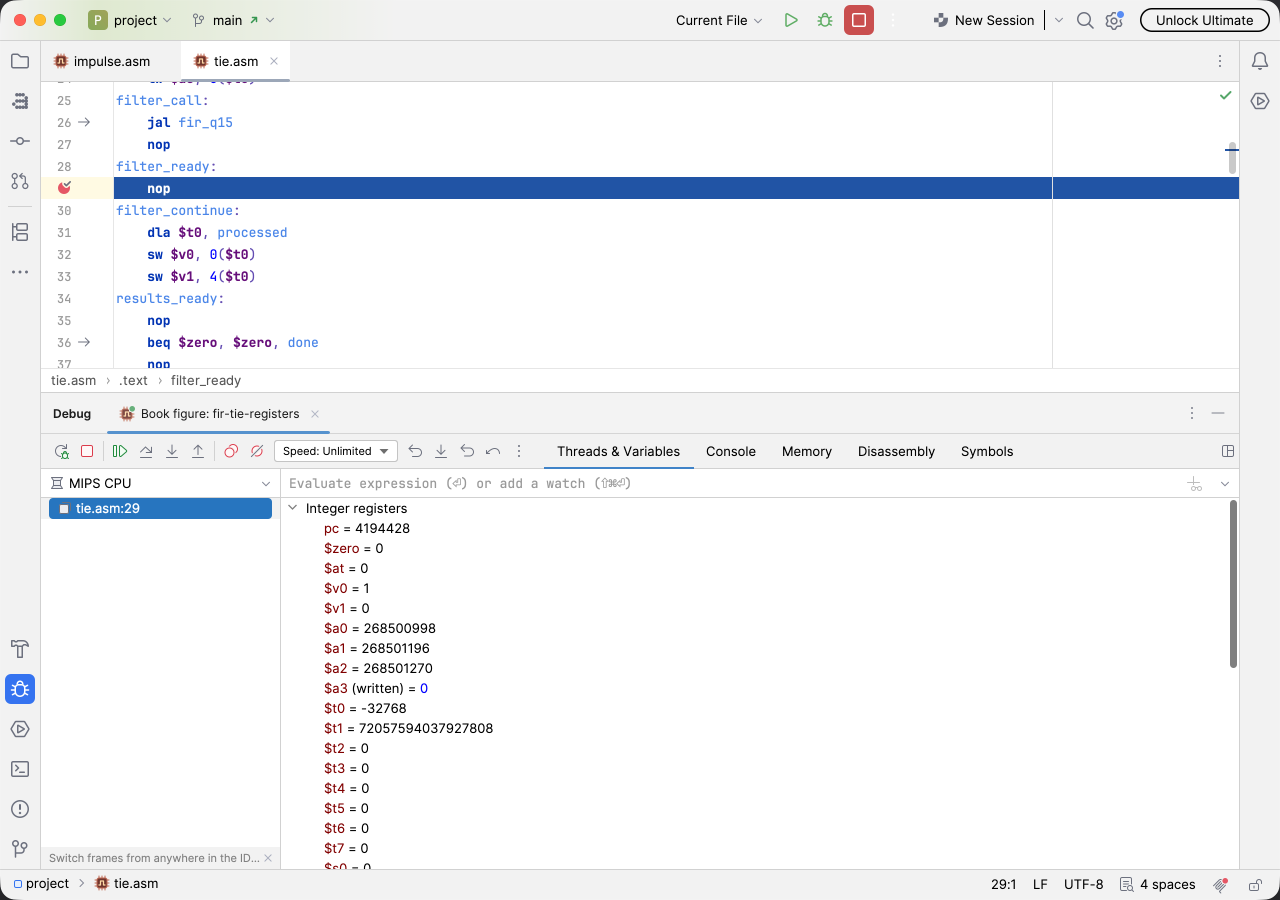
\includegraphics[width=0.42\linewidth,artifact,trim={\MARSfirtieregistersLeft{} \MARSfirtieregistersBottom{} \MARSfirtieregistersRight{} \MARSfirtieregistersTop{}},clip]{book/captures/021-fixed-point-fir/f03/registers.png}};
    \begin{scope}[shift={(registers.south west)},x={($(registers.south east)-(registers.south west)$)},y={($(registers.north west)-(registers.south west)$)}]
      \draw[black,line width=0.7pt] (0.023437500,0.023255814) rectangle (0.218750000,0.953488372);
      \node[draw=black,fill=white,circle,inner sep=1.5pt,font=\footnotesize] at ($(0.023437500,0.953488372)+(-3mm,0)$) {2};
    \end{scope}
    \node[anchor=north west,inner sep=0,font=\small\bfseries] (input-title) at ([yshift=-1mm]source.south west) {Input window detail};
    \node[anchor=north west,inner sep=0] (input) at ([yshift=-1mm]input-title.south west) {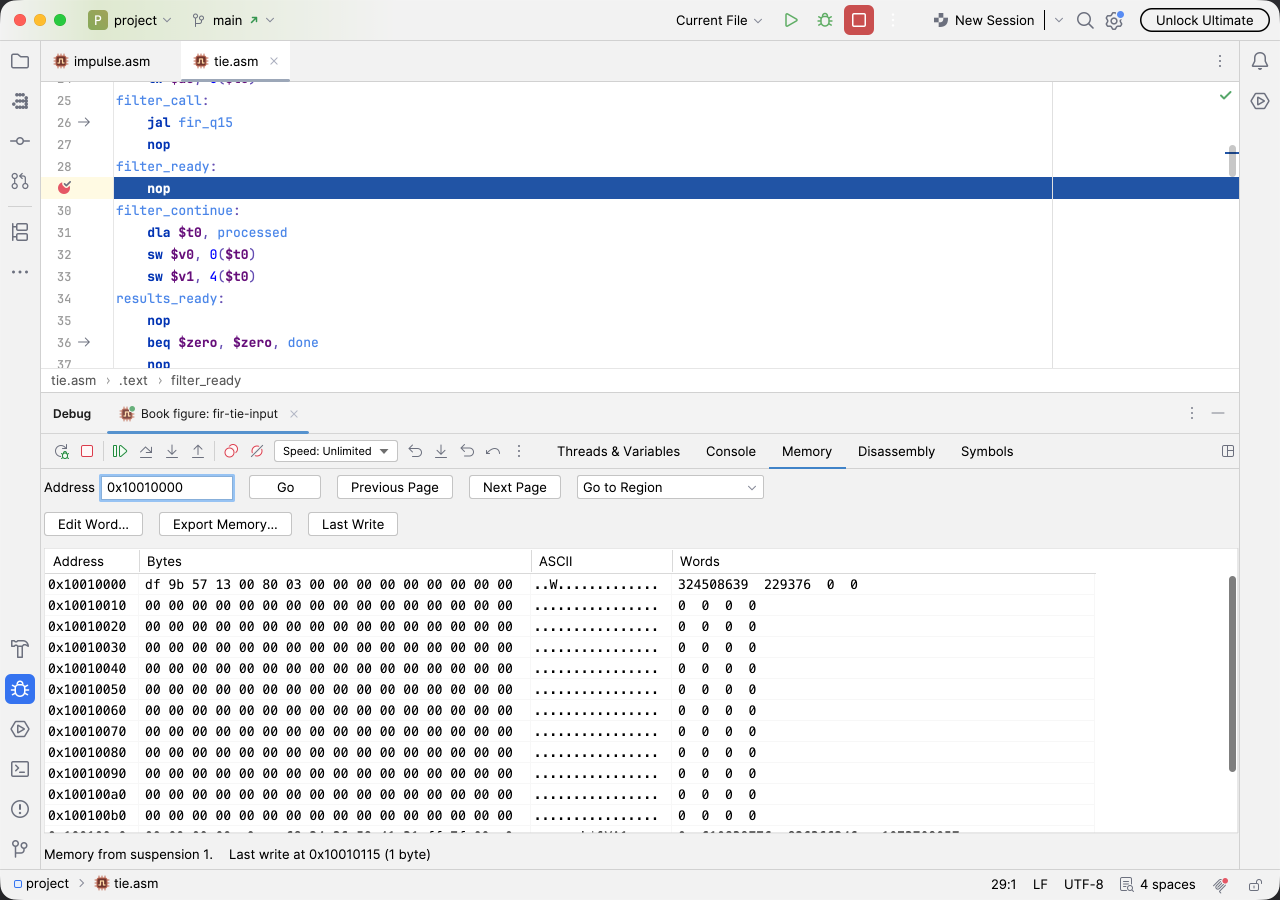
\includegraphics[width=0.84\linewidth,artifact,trim={\MARSfirtieinputLeft{} \MARSfirtieinputBottom{} \MARSfirtieinputRight{} \MARSfirtieinputTop{}},clip]{book/captures/021-fixed-point-fir/f03/input.png}};
    \begin{scope}[shift={(input.south west)},x={($(input.south east)-(input.south west)$)},y={($(input.north west)-(input.south west)$)}]
      \draw[black,line width=0.7pt] (0.194672131,0.055555556) rectangle (0.997950820,0.638888889);
      \node[draw=black,fill=white,circle,inner sep=1.5pt,font=\footnotesize] at ($(0,0.638888889)+(-3mm,0)$) {3};
    \end{scope}
    \node[anchor=north west,inner sep=0,font=\small\bfseries] (coefficients-title) at ([yshift=-1mm]input.south west) {Eight signed coefficient codes};
    \node[anchor=north west,inner sep=0] (coefficients) at ([yshift=-1mm]coefficients-title.south west) {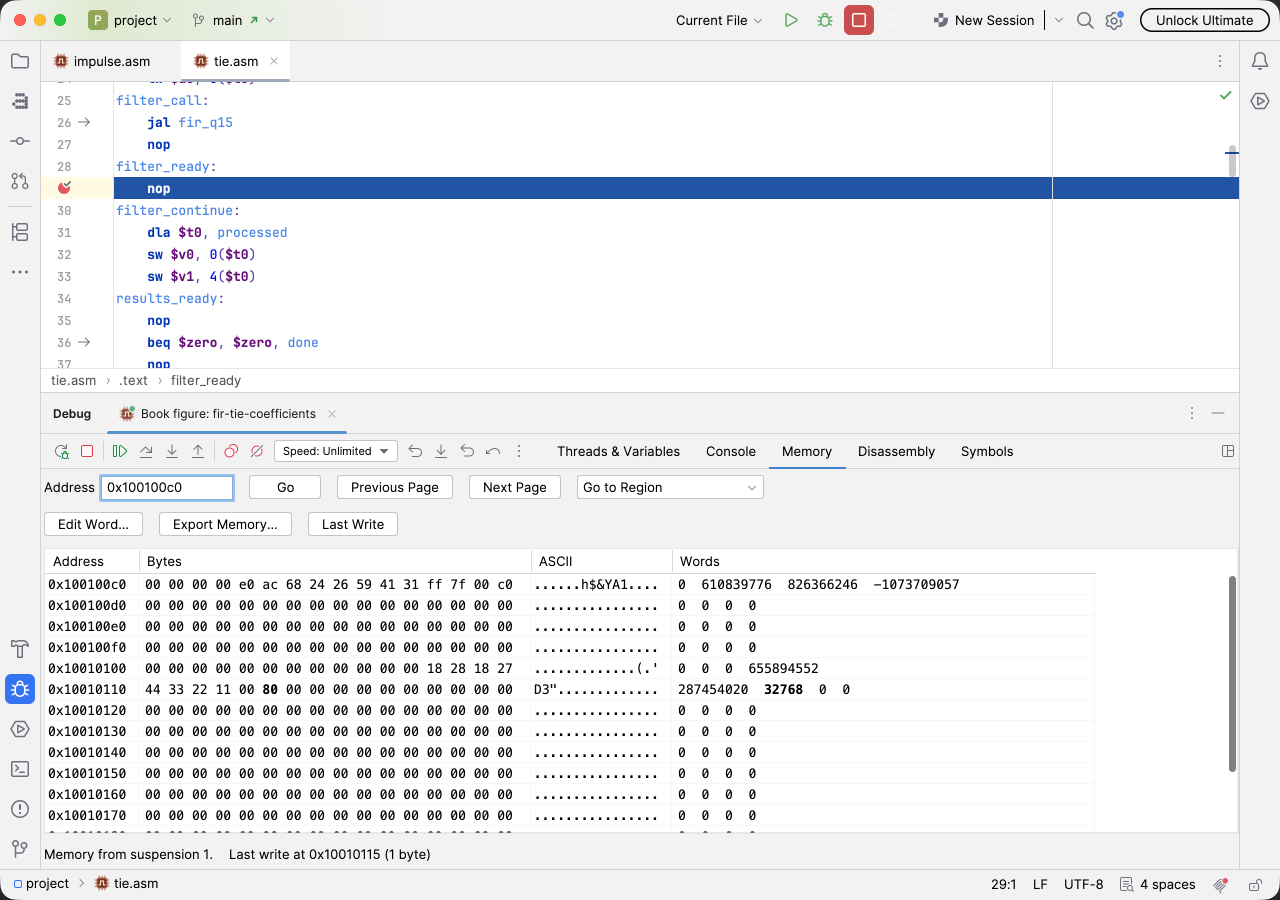
\includegraphics[width=0.84\linewidth,artifact,trim={\MARSfirtiecoefficientsLeft{} \MARSfirtiecoefficientsBottom{} \MARSfirtiecoefficientsRight{} \MARSfirtiecoefficientsTop{}},clip]{book/captures/021-fixed-point-fir/f03/coefficients.png}};
    \begin{scope}[shift={(coefficients.south west)},x={($(coefficients.south east)-(coefficients.south west)$)},y={($(coefficients.north west)-(coefficients.south west)$)}]
      \draw[black,line width=0.7pt] (0.194672131,0.055555556) rectangle (0.997950820,0.638888889);
      \node[draw=black,fill=white,circle,inner sep=1.5pt,font=\footnotesize] at ($(0,0.638888889)+(-3mm,0)$) {4};
    \end{scope}
    \node[anchor=north west,inner sep=0,font=\small\bfseries] (output-title) at ([yshift=-1mm]coefficients.south west) {Selected output halfwords};
    \node[anchor=north west,inner sep=0] (output) at ([yshift=-1mm]output-title.south west) {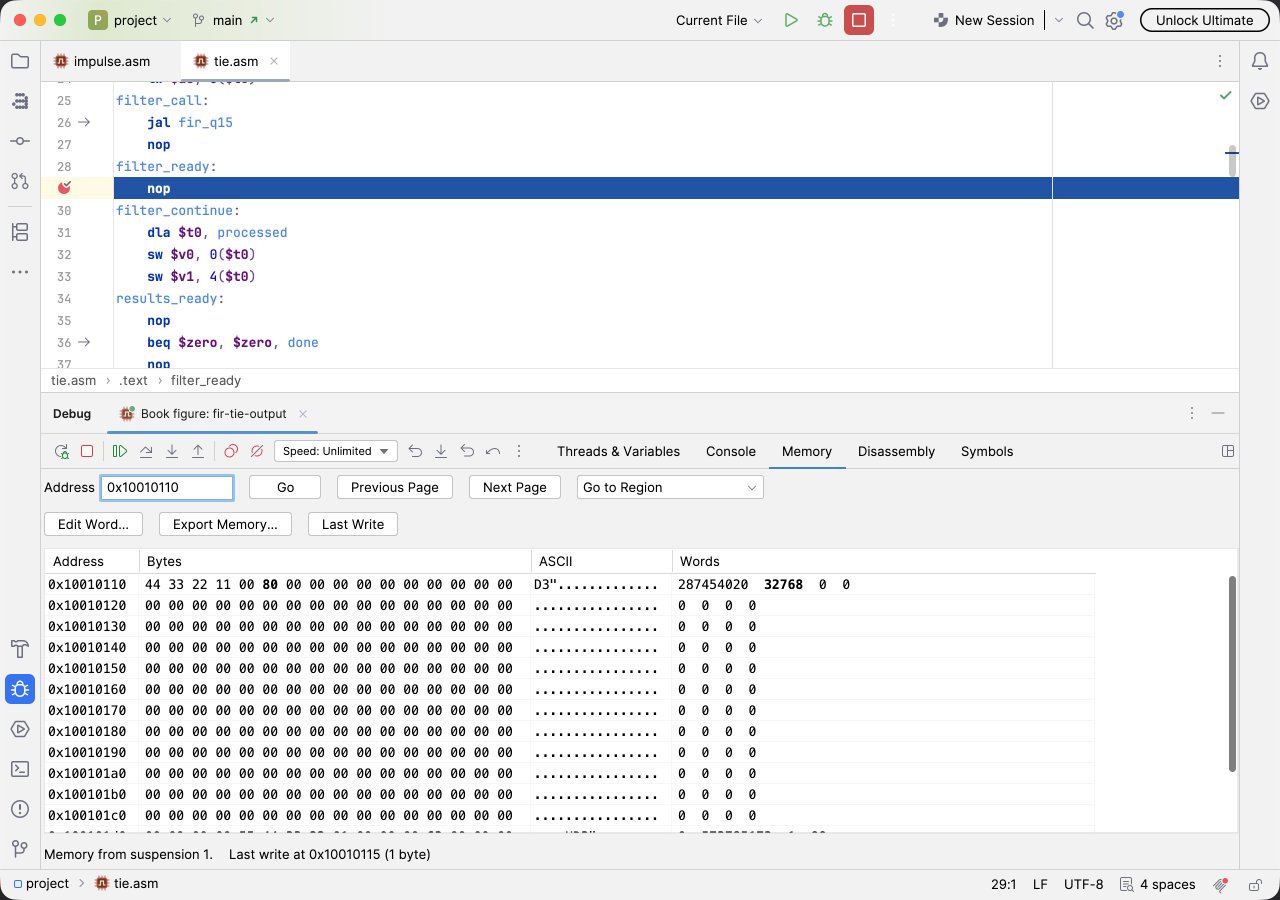
\includegraphics[width=0.84\linewidth,artifact,trim={\MARSfirtieoutputLeft{} \MARSfirtieoutputBottom{} \MARSfirtieoutputRight{} \MARSfirtieoutputTop{}},clip]{book/captures/021-fixed-point-fir/f03/output.png}};
    \begin{scope}[shift={(output.south west)},x={($(output.south east)-(output.south west)$)},y={($(output.north west)-(output.south west)$)}]
      \draw[black,line width=0.7pt] (0.194672131,0.078431373) rectangle (0.997950820,0.490196078);
      \node[draw=black,fill=white,circle,inner sep=1.5pt,font=\footnotesize] at ($(0,0.490196078)+(-3mm,0)$) {5};
    \end{scope}
    \node[anchor=north west,inner sep=0,font=\small\bfseries] (caller-title) at ([yshift=-1mm]output.south west) {Count and saved caller results};
    \node[anchor=north west,inner sep=0] (caller) at ([yshift=-1mm]caller-title.south west) {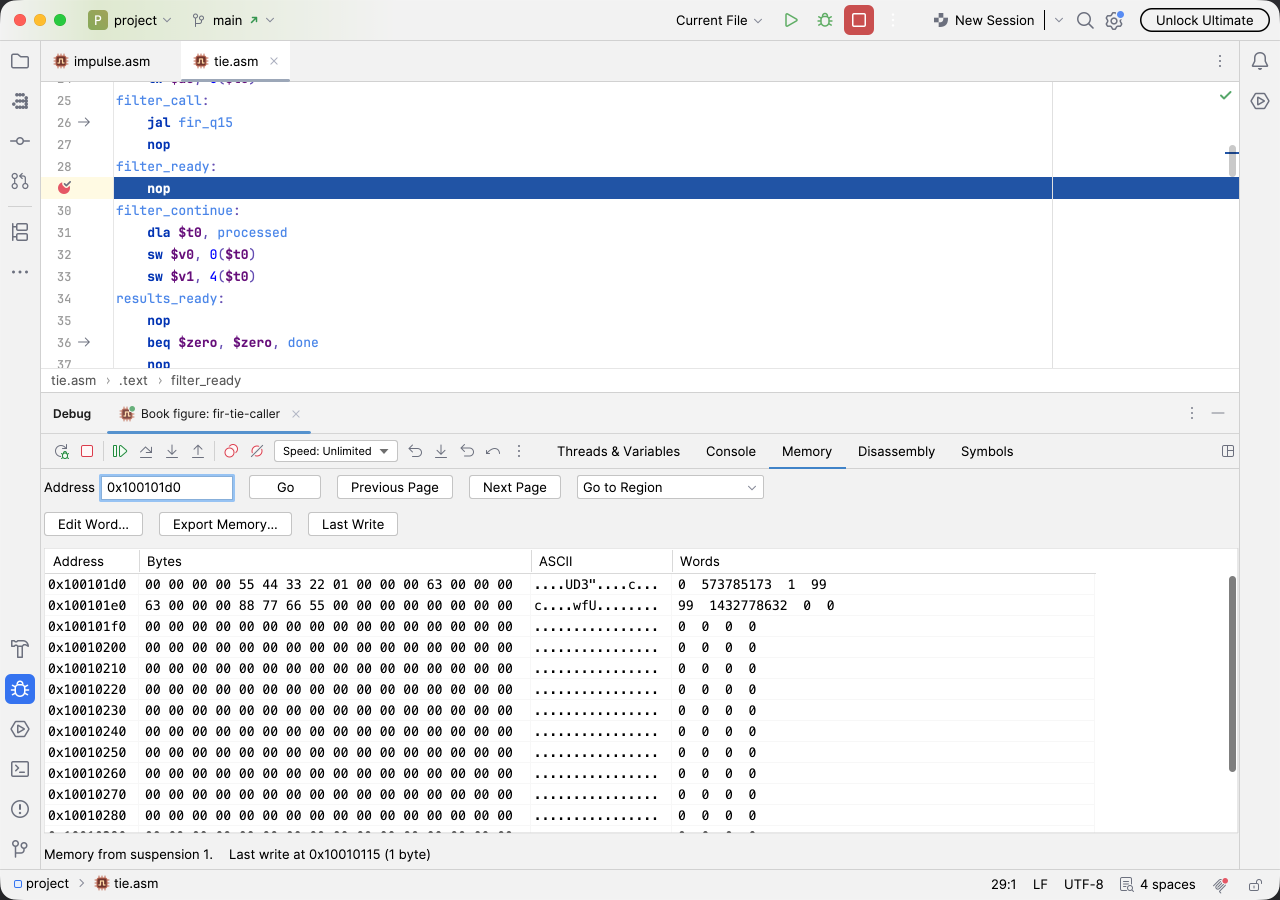
\includegraphics[width=0.84\linewidth,artifact,trim={\MARSfirtiecallerLeft{} \MARSfirtiecallerBottom{} \MARSfirtiecallerRight{} \MARSfirtiecallerTop{}},clip]{book/captures/021-fixed-point-fir/f03/caller.png}};
    \begin{scope}[shift={(caller.south west)},x={($(caller.south east)-(caller.south west)$)},y={($(caller.north west)-(caller.south west)$)}]
      \draw[black,line width=0.7pt] (0.194672131,0.055555556) rectangle (0.997950820,0.638888889);
      \node[draw=black,fill=white,circle,inner sep=1.5pt,font=\footnotesize] at ($(0,0.638888889)+(-3mm,0)$) {6};
    \end{scope}
  \end{tikzpicture}
  \par\smallskip
  \begin{minipage}{\linewidth}
    \small
    \begin{enumerate}
      \setlength{\itemsep}{2pt}
            \setlength{\parsep}{0pt}
      \item This one-output fixture uses eight input samples, including seven history samples. The stop remains \texttt{filter\_ready}, after rounding and saturation checks but before the caller stores its results.
      \item \texttt{\$v0 = 1} and \texttt{\$v1 = 0}. Clipping is tested on the rounded integer. A rounded value equal to $-32768$ is representable and contributes zero to the clipping count.
      \item The first two input codes are $-32768$ (\texttt{00 80}) and 3 (\texttt{03 00}); the remaining six are zero. Their order is oldest to newest within the supplied window.
      \item The first two coefficients are 32767 (\texttt{ff 7f}) and $-16384$ (\texttt{00 c0}); the rest are zero. The exact accumulator is $-1073758208$, or $-32768.5$ after Q15 scaling. The halfway rule selects the greater neighboring integer, $-32768$.
      \item The output halfword at \texttt{0x10010114} is \texttt{00 80}, encoding $-32768$. That endpoint value by itself does not establish clipping. Here rounding already produced a representable value.
      \item Count is 1, and both caller result words remain 99. The next stores will publish processed 1 and clipped 0. The live second return supplies the distinction between this case and the following clipped endpoint.
    \end{enumerate}
  \end{minipage}
  \caption{A negative halfway value rounds to the minimum halfword without clipping.}
  \label{capture:021-fixed-point-fir-f03}
  \label{fir-f03}
\end{figure}
\par
